%!TEX ROOT=../emnlp2023.tex

% show figures/pipeline.png


\section{Introduction}
\label{sec:introduction}
In 2024, Automated Verification of Textual Claims (AVeriTeC) shared task~\cite{schlichtkrull-etal-2024-automated} shown that the fact-checking of real-world claims like those from Politifact, AfricaCheck, etc., can be automated to a significant extent, with pipelines accessing Large Language Models (LLMs) to produce the evidence and veracity verdicts for previously unseen claims instead of a human.
Almost each competitive AVeriTeC shared-task system, however, relied on a proprietary LLM like GPT-4o~\cite{rothermel-etal-2024-infact,ullrich-etal-2024-aic} or an open-weights model with high tens of billions of parameters~\cite{yoon-etal-2024-hero}.
This raised a concern -- can the fact-checking process be automated in a way accessible to masses, or is its quality conditioned by the business-owned blackbox models or access to prohibitive computational resources?

In this year's~\averitec{} shared task, the challenge is to match the quality of AVeriTeC systems with ones that only use open-weights models, constrained time of 60 seconds per claim on average, and a fixed compute of a single 20GB A10 GPU.

Our AIC CTU system (Figure~\ref{fig:pipeline}), adapted for \averitec{} from our last year submission, tops its test-leaderboard (Table~\ref{tab:leaderboard}) with a simple Retrieval-augmented Generation (RAG) scheme, using a locally hosted (Ollama) instance of Qwen3 LLM with 14B params, leveraging the sheer context length modern day LLMs can process.

%\vspace{-.5em}
\begin{minipage}{\linewidth}
    \centering
    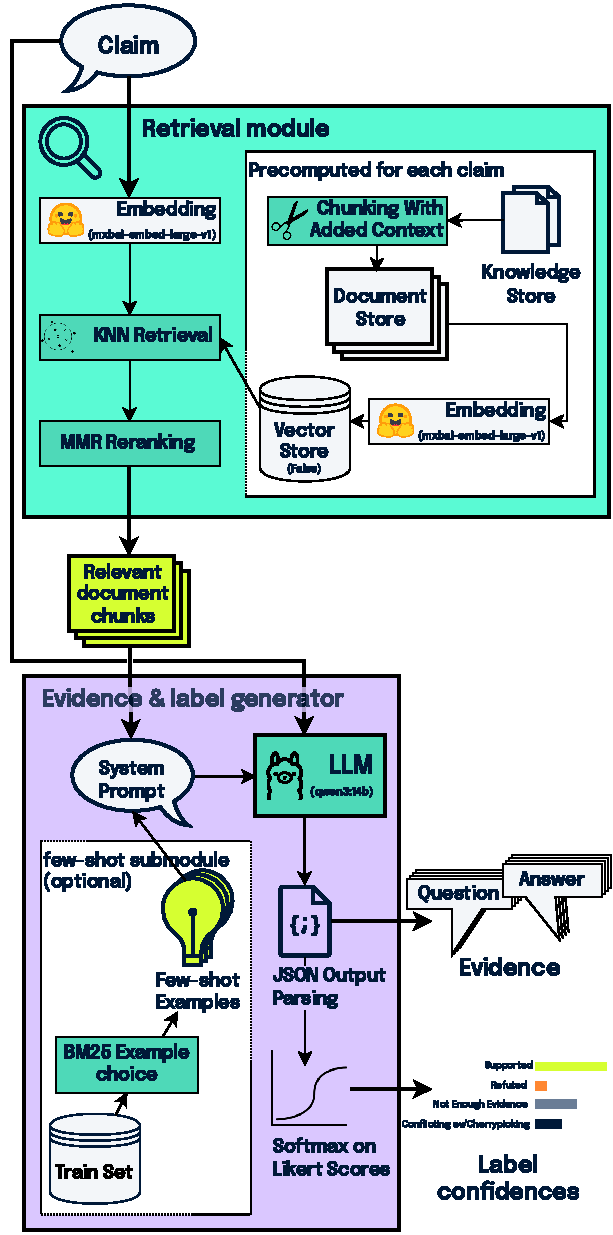
\includegraphics[width=\linewidth]{figures/pipeline.pdf}
    \captionof{figure}{Our refreshed fact-checking pipeline used in CTU AIC FEVER 8 submission, adapted from~\citealt{ullrich-etal-2024-aic}.}
    \label{fig:pipeline}
\end{minipage}

This paper introduces our system, discusses its design choices and how do they account on the score.
We suggest our system as the new strong baseline -- simple at core, competitive results -- providing the code and reproduction advice.

%\section{Related work}
\label{sec:relwork}
\label{avscore}
%\begin{enumerate}
%    \item \textbf{\averitec{} shared task}~\cite{averitec2024} releases the datase of real-world fact-checked claims, annotated with evidence available at the date the claim was made.
%\end{enumerate}

